%%%%%%%%%%%%%%%%%%%%%%%%%%% COORDINATESYSTEMS
% COORDSYS (ORIGOCOORDINATENAME, WIDTH, HEIGHT)
% Draws a Coordinatesystem around ORIGOCOORDINATENAME with a width of WIDTH and a height of HEIGHT, 
% names the beginning and end of axes, southwest corner, northwest corner, 
\newcommand{\ThreeDimCoordSys}[4]{
\coordinate (XY#1) at ([xshift=#2 cm, yshift=#3 cm]#1);
\coordinate (-XY#1) at ([xshift=-#2 cm, yshift=-#3 cm]#1);
\coordinate (X#1) at ([xshift=#2 cm]#1);
\coordinate (-X#1) at ([xshift=-#2 cm]#1);
\coordinate (Y#1) at ([yshift=#3 cm]#1);
\coordinate (-Y#1) at ([yshift=-#3 cm]#1);
%\path (#1); \pgfgetlastxy{\XCoord}{\YCoord}; % Extracting coordinates of the Origin
%\pgfmathsetmacro{\XCoordcm}{\XCoord/28.4527}
%\pgfmathsetmacro{\YCoordcm}{\YCoord/28.4527}
%\coordinate (Z#1) at (\XCoordcm, \YCoordcm,#4);
%\coordinate (-Z#1) at (\XCoordcm, \YCoordcm,-#4);
%\draw [help lines, step=.5cm] (-XY#1) grid (XY#1);
\coordinate (Z#1) at ([shift=(\ThirdAxisAngle : #4*\ThirdAxisUnit cm)]#1);
\coordinate (-Z#1) at ([shift=(\ThirdAxisAngle : #4*\ThirdAxisUnit cm)]#1);
\draw[->, name path=XAxis#1] (#1)--(X#1);
\draw[->, name path=YAxis#1] (#1)--(Y#1);
\draw[->, name path=ZAxis#1] (#1)--(Z#1);
}

% \DistanceLabel{SS}{AS}{-45}{1}{pos=.5}{1}
\newcommand{\DistanceLabel}[6]{
\coordinate(#1horgony) at ([shift=(#3:#4)] #1);
\coordinate(#2horgony) at ([shift=(#3:#4)] #2);
\draw[thin, red, <->] (#1horgony)--(#2horgony) node[#5]{#6};
\draw[opacity=.4, black] (#1)--(#1horgony);
\draw[opacity=.4, black] (#2)--(#2horgony);
}

%Lorentz(OriginalOriginCoord, ResultingOriginCoord, SpeedNum, PointCoord, Label)
% 
\newcommand{\Lorentz}[5]{
\path (#1); \pgfgetlastxy{\XCoord}{\YCoord}; % Extracting coordinates of the Origin
\pgfmathsetmacro{\XOrigin}{\XCoord} % Saving X coordinate
\pgfmathsetmacro{\YOrigin}{\YCoord} % Saving Y coordinate
\path (#4); \pgfgetlastxy{\XCoord}{\YCoord}; % Extracting coordinates of the Point
\pgfmathsetmacro{\XEvent}{\XCoord} % Saving X coordinate
\pgfmathsetmacro{\YEvent}{\YCoord} % Saving Y coordinate
\pgfmathsetmacro{\XEventWRTOrigin}{\XEvent-\XOrigin} % Relativizing to the origin
\pgfmathsetmacro{\YEventWRTOrigin}{\YEvent-\YOrigin} % Relativizing to the origin
\pgfmathparse{XLorentz(#3,\XEventWRTOrigin,\YEventWRTOrigin)} % transforming x
\pgfmathsetmacro{\XEventTr}{\pgfmathresult} % save the result of x
\pgfmathparse{YLorentz(#3,\XEventWRTOrigin,\YEventWRTOrigin)} % transforming y
\pgfmathsetmacro{\YEventTr}{\pgfmathresult} % save the result of y
\node[world](#5) at (
[xshift=\XEventTr pt,
 yshift=\YEventTr pt] #2){};
}

\usetikzlibrary{calc}
\usetikzlibrary{intersections}
\newdimen\XCoord
\newdimen\YCoord

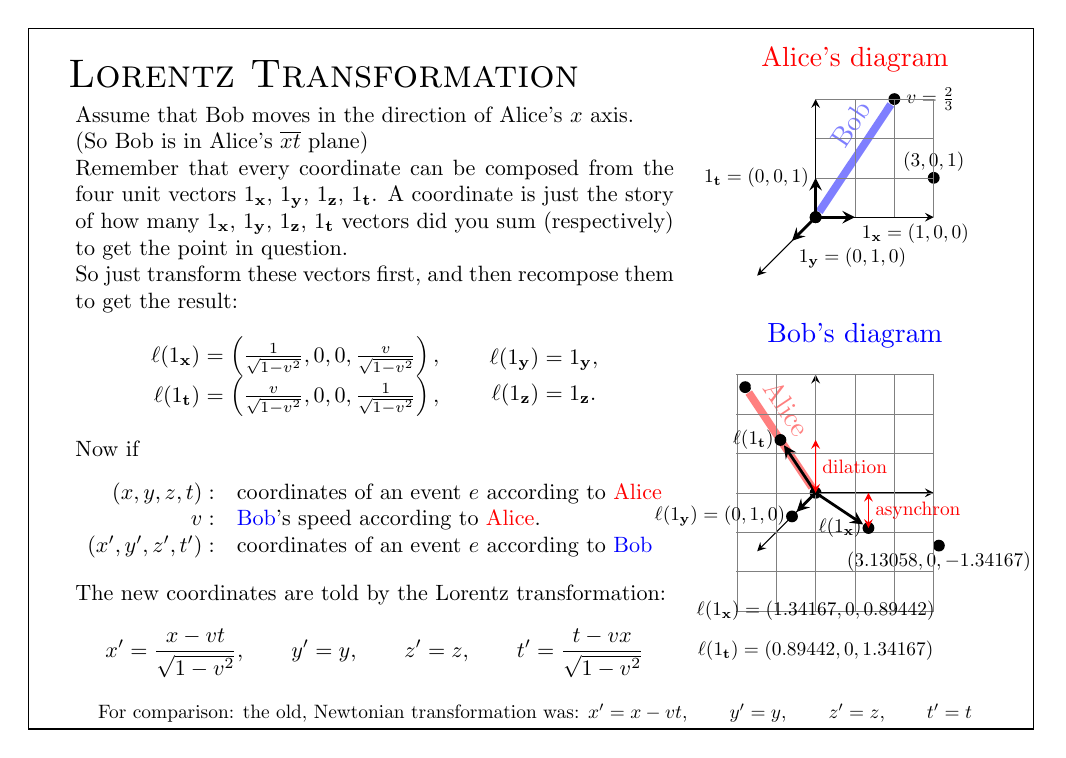
\begin{tikzpicture}[>=stealth, scale=1,
world/.style={inner sep=0, minimum size=.15cm, fill=black, circle},
worldline/.style={line width=1mm, rounded corners=1pt, opacity=.5},
axis/.style={->},
light/.style={orange, line width=.5mm},
]
\pgfmathdeclarefunction{XLorentz}{3}{\pgfmathparse{(#2 - #1*#3)/(sqrt(1-#1^2))}} % speed, spacecoord, timecoord
\pgfmathdeclarefunction{YLorentz}{3}{\pgfmathparse{(#3 - #1*#2)/(sqrt(1-#1^2))}} % speed, spacecoord, timecoord
\pgfmathsetmacro{\ThirdAxisAngle}{-135}
\pgfmathsetmacro{\ThirdAxisUnit}{.7}

%%%%%%%%%%%%%%%%%%%%%%%% DIA KEZDETE %%%%%%%%%%%%%%%%%%%%%%%%%%%

\node[anchor=north west, inner sep=0] at (0.5,8.5) {\textsc{\Large Lorentz Transformation}}; %%%%%%% TITLE
%\node[anchor=north west, inner sep=0] at (0.5,8) {\textsc{\normalsize Role of Light}}; %%%%%%% SUBTITLE
\draw%[white]  %%%%%%%%%%%% SIZE OF THE SLIDE
      (0,0) rectangle (12.77,8.9);
%%%%%%%%% TEXT %%%%%%%%%%%%%
\node[anchor=north west, scale=.8] at (0.5,8) {\begin{minipage}{9.5cm}
Assume that Bob moves in the direction of Alice's $x$ axis. 
\\ (So Bob is in Alice's $\overline{xt}$ plane)

Remember that every coordinate can be composed from the four unit vectors
$1_{\mathbf x}$, $1_{\mathbf y}$, $1_{\mathbf z}$, $1_{\mathbf t}$. 
 {A coordinate is just the story of how many $1_{\mathbf x}$, $1_{\mathbf y}$, $1_{\mathbf z}$, $1_{\mathbf t}$ vectors did you sum (respectively) to get the point in question.}

So just transform these vectors first, and then recompose them to get the result:
\[\arraycolsep=.5mm\begin{array}{rcl}
\ell (1_{\mathbf x}) &=& \left( \frac 1{\sqrt{1-v^2}}, 0,0,\frac v{\sqrt{1-v^2}}\right),
\\ \ell (1_{\mathbf t}) &=& \left( \frac v{\sqrt{1-v^2}}, 0,0,\frac 1{\sqrt{1-v^2}}\right),
\end{array}\qquad
\begin{array}{rcl}
 \ell (1_{\mathbf y}) &=& 1_{\mathbf y},
\\[1ex] \ell (1_{\mathbf z}) &=& 1_{\mathbf z}.
\end{array}
\]
Now if 
\[\begin{array}{rl}
(x,y,z,t) : & \textup{coordinates of an event $e$ according to \textcolor{red}{Alice}}
\\ v: & \textup{\textcolor{blue}{Bob}'s speed according to \textcolor{red}{Alice}}.  
\\ (x',y',z',t'): & \textup{coordinates of an event $e$ according to \textcolor{blue}{Bob}} 
\end{array}
\]
The new coordinates are told by the Lorentz transformation:
%\[\begin{array}{rcl}
%    x'&=&\frac{x-vt}{\sqrt{1-v^2}}
%\\ y'&=& y
%\\ z'&=& z
%\\ t'&=&\frac{t-vx}{\sqrt{1-v^2}}
%\end{array}\]
\[x'=\frac{x-vt}{\sqrt{1-v^2}}, \qquad y'=y, \qquad z'=z,\qquad t'=\frac{t-vx}{\sqrt{1-v^2}}\]
\end{minipage}
};
%%%%%%%%%%%%%%%%%%%%%%%% KOORDINÁTARENDSZEREK %%%%%%%%%%%%%%%%%%%%%%%%%%%
\coordinate(O1) at (10,6.5) {} {} {} {} {} {} {};
  \ThreeDimCoordSys{O1}{1.5}{1.5}{1.5}
\coordinate(O2) at (10,3) {} {} {} {} {} {} {} {};
  \ThreeDimCoordSys{O2}{1.5}{1.5}{1.5}

%%%%%%%%%%
%% SETTINGS %%
%%%%%%%%%%

\coordinate (AliceStart) at (O1);
\coordinate (AliceEnd) at (10,7.5) {} {} {} {} {} {} {} {} {} {} {};
\coordinate (BobStart) at (O1); % Fontos hogy átmenjen az Origón, különben rossz a lorentz transzformáció!!
\coordinate (BobEnd) at (11,8) {} {} {} {} {} {} {} {} {} {} {} {} {};

%%%%%%%%%%% Ezt lehetne macronak, speedszámítócuccnak
\path (BobStart); \pgfgetlastxy{\XCoord}{\YCoord}; % Extracting coordinates of the Origin
\pgfmathsetmacro{\XFirst}{\XCoord} % Saving X coordinate
\pgfmathsetmacro{\YFirst}{\YCoord} % Saving Y coordinate
\path (BobEnd); \pgfgetlastxy{\XCoord}{\YCoord}; % Extracting coordinates of the Point
\pgfmathsetmacro{\XSecond}{\XCoord} % Saving X coordinate
\pgfmathsetmacro{\YSecond}{\YCoord} % Saving Y coordinate
\pgfmathsetmacro{\SpeedBob}{(\XFirst-\XSecond)/(\YFirst-\YSecond)} % Relativizing to the origin
%%%%%%%%%%%%%%%%%%%%%%%%%%%%%%%%%%%

\Lorentz{O1}{O1}{0}{BobStart}{BS}
\Lorentz{O1}{O1}{0}{BobEnd}{BE}
\Lorentz{O1}{O1}{0}{AliceStart}{AS}
%\Lorentz{O1}{O1}{0}{AliceEnd}{AE}
\Lorentz{O1}{O2}{\SpeedBob}{AliceStart}{AS'}
\Lorentz{O1}{O2}{\SpeedBob}{AliceEnd}{AE'}
\node[world] (e) at (11.5,7) {};
%\node[anchor=south] at (e) {$(x,y,z,t)$};
\node[anchor=south, scale=.7] at (e) {$(3,0,1)$};
\node[anchor=west, scale=.7, inner sep=6] at (BobEnd) {$v=\frac 23$};
\Lorentz{O1}{O2}{\SpeedBob}{e}{e'}
%\node[anchor=north] at (e') {$\left(\frac{x-vt}{\sqrt{1-v^2}}, y, z, \frac{t-vx}{\sqrt{1-v^2}}\right)$};

\pgfmathsetmacro{\X}{(3 - 1*2/3)/(sqrt(1-(2/3)^2))}
\pgfmathsetmacro{\T}{(1 - 3*2/3)/(sqrt(1-(2/3)^2))}
\node[anchor=north, scale=.7] at (e') {$\left( \X, 0, \T\right)$};

\node[rotate=0, text=red, fill=white] at (10.5,8.5) {Alice's diagram};
\node[rotate=0, text=blue, fill=white] at (10.5,5) {Bob's diagram};
\draw[worldline, blue] (BS)--(BE) node[fill=white, sloped, above, pos=.7]{Bob};
\draw[worldline, red] (AS')--(AE') node[fill=white, sloped, above, pos=.7]{Alice};

%\node[scale=.7] at (10,1) {\begin{minipage}{5cm}The illustration is faithful for 
%
%\vspace{-1em}
%\[(x,y,z,t)= (3,0,0,1)\]\end{minipage}};
\coordinate (v1) at (10,7) {};
\coordinate (v2) at (10.5,6.5) {};
\coordinate (v3) at (9.70,6.20) {};
\begin{scope}[line width=1]
\draw[->]  (O1) -- (v1);
\draw[->]  (O1) -- (v2);
\draw[->]  (O1) -- (v3);
\end{scope}
\node[scale=.7, anchor=east] at (v1){$1_{\mathbf t} = (0,0,1)$};
\node[scale=.7, anchor=north west] at (v2){$1_{\mathbf x} = (1,0,0)$};
\node[scale=.7, anchor=north west] at (v3){$1_{\mathbf y} = (0,1,0)$};
\draw [help lines, step=.5cm] (O1) grid (XYO1);
\draw [help lines, step=.5cm] ([yshift=-1.501cm, xshift=-1.01cm]O2) grid (XYO2);
\Lorentz{O1}{O2}{\SpeedBob}{v1}{v1'}
\Lorentz{O1}{O2}{\SpeedBob}{v2}{v2'}
\Lorentz{O1}{O2}{0}{v3}{v3'}
\begin{scope}[line width=1]
\draw[->]  (O2) -- (v1');
\draw[->]  (O2) -- (v2');
\draw[->]  (O2) -- (v3');
\end{scope}
\pgfmathsetmacro{\X}{1/(sqrt(1-(2/3)^2))}
\pgfmathsetmacro{\T}{(2/3)/(sqrt(1-(2/3)^2))}
\node[scale=.7, anchor=east] at (v1') {$\ell(1_{\mathbf t})$};
\node[scale=.7, anchor=east] at (v2') {$\ell(1_{\mathbf x})$};
\node[scale=.7] at (10,1) {$\ell(1_{\mathbf t}) = (\T,0,\X)$};
\node[scale=.7] at (10,1.5) {$\ell(1_{\mathbf x}) = (\X,0,\T)$};
\node[scale=.7, anchor=east] at (v3'){$\ell(1_{\mathbf y}) = (0,1,0)$};
\coordinate(refx) at ([yshift=1cm]v2');
\coordinate(reft) at ([xshift=1cm]v1');
\path[name path=myvertical] (v2')--(refx);
\path[name path=myhorizontal] (v1')--(reft);
\node[inner sep=0,name intersections={of=myvertical and XAxisO2, by=vetx}] at (vetx){};
\node[inner sep=0,name intersections={of=myhorizontal and YAxisO2, by=vett}] at (vett){};
\DistanceLabel{v2'}{vetx}{0}{0 mm}{pos=.5, right, scale=.7}{asynchron}
\DistanceLabel{O2}{vett}{0}{0 mm}{pos=.5, right, scale=.7}{dilation}
\node[scale=.7, anchor=west] at (0.8,0.2) {For comparison: the old, Newtonian transformation was:
%\[\begin{array}{rcl}
%    x'&=& x-vt
%\\ y'&=& y
%\\ z'&=& z
%\\ t'&=& t
%\end{array}\]
$x'=x-vt, \qquad y'=y, \qquad z'=z,\qquad t'=t$
};
\end{tikzpicture}